\section{Context-free Languages}
\subsection{Introduction}
Basic example of a non-regular language: $L$ is composed of all words starting with $a$'s
and ending with the same number of $b$'s:
\begin{align*}
  L=\{a^n b^n \mid n \geq 0\}
\end{align*}
This language cannot be recognized by a FSA,
nor generated by a regular grammar,
nor denoted by a regular expression.
The limitation comes from the fact that FSA
have a finite set of states. Consequently,
FSA cannot memorize and arbitrary large number n 
of symbols $a$ and verify that the same number of $b$ follows.\\

Non-regular languages include:
\begin{itemize}
  \item Nested paranthesis in arithmetic expressions
  \item Nested \texttt{begin}, \texttt{end} in programming languages
  \item Nested \texttt{\textbraceleft} and \texttt{\textbraceright} in programming languages
  \item And a lot more\dots
\end{itemize}
\textit{Example (Stack):} FSA cannot be used to model
a stack with the operations push and pop, for which the number 
of push operations is arbitrarily large.
\begin{figure}[H]
  \centering
  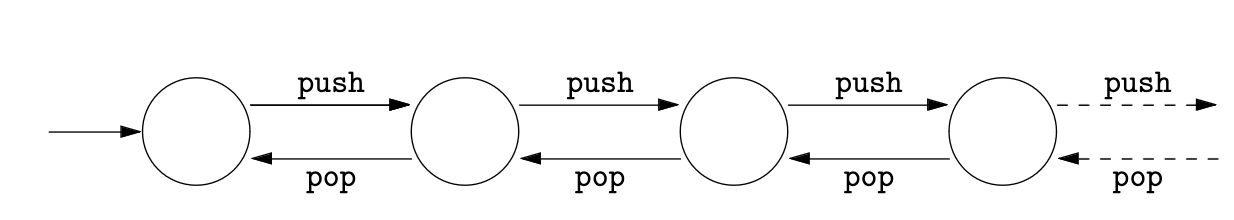
\includegraphics[width=\columnwidth]{context-free-1}
\end{figure}
Note that if a language $L$ is non-regular,
a language $L \subset L'$ is not necessarily non-regular:
\textit{Example:} The left-hand side language is non-regular,
whereas the right-hand side language is regular:

\begin{align*}
  \{ a^{n} , b^{n} \mid n \geq 0 \} \subset \{ a , b \}^{*}
\end{align*}

The distinguishing characteristic is the structure.
\subsection{Pushdown Automata}
To overcome some limitations of FSA, \textbf{pushdown automata} have been devised:
\begin{itemize}
  \item A pushdown automaton (PDA) is a kind of finite state automaton equipped with a stack that memorizes symbols.
  \item The transitions of a pushdown depend on an input symbol but also on the symbol at the top of the stack.
  \item The size of the stack has no limit.
\end{itemize}
\textit{Example: } Using the previous language $\{a^n b^n \mid n \geq 1\}$, the PDA behaves as follows:
\begin{enumerate}
  \item While a symbol can be read, this symbol is pushed onto the stack.
  \item When the first input symbol $b$ comes, then one symbol $a$ is removed from the stack.
  \item While a symbol $b$ can be read, one symbol $a$ is removed from the stack.
  \item The process ends when the stack is empty and all the input symbols have been consumed.
\end{enumerate}
Formal definition: A pushdown automaton PDA is a 6-tuple $M = (Q,\Sigma,\Gamma,\delta,q_0,\triangleleft)$, where:
\begin{itemize}
  \item $Q$ is a finite set of states
  \item $\Sigma$ is an input alphabet
  \item $\Gamma$ is an auxiliary alphabet (symbols of the stack) such that $\Gamma \cap \Sigma = \emptyset$ (i.e. $\Gamma$ and $\Sigma$ share no elements)
  \item $\delta : Q \times (\Sigma \cup \{\epsilon\}) \times \Gamma \rightarrow Q \times \Gamma^{*}$ is a transition function
  \item $q_0 \in Q$ is the initial state
  \item $\triangleleft \in \Gamma$ is a special symbol which indicates that the stack is empty
\end{itemize}
A PDA that recognizes a language is defined similarly: We add the set of final states.
This means that a recognizer is a 7-tuple $M = (Q,\Sigma,\Gamma,\delta,q_0,\triangleleft,F)$ ,
where $F \subseteq Q$ is the set of final states.\\

\textit{Example:} Let us construct a PDA $M$ which recognizes $a^n b^n \mid n \geq 1$:
\begin{align*}
  M = (\{q_0, q_1, q_2\}, \{a,b\}, \{A,\triangleleft\}, q_0, \triangleleft, \{q_2\})
\end{align*}
where
\begin{align*}
  \delta(q_0, a, \triangleleft) = (q_0, A\triangleleft)\\
  \delta(q_0, a, A) = (q_0, AA)\\
  \delta(q_0, b, A) = (q_1, \epsilon)\\
  \delta(q_1, b, A) = (q_1, \epsilon)\\
  \delta(q_0, \epsilon, \triangleleft) = (q_2, \epsilon)\\
\end{align*}
Convention: $(a, Z \mid \alpha)$ means:
\begin{itemize}
  \item $a$ is the input symbol
  \item $Z$ is the symbol at the top of the stack before applying the transition function
  \item $\alpha$ is the content of the stack after the application of the transition function
\end{itemize}
\begin{figure}[H]
  \centering
  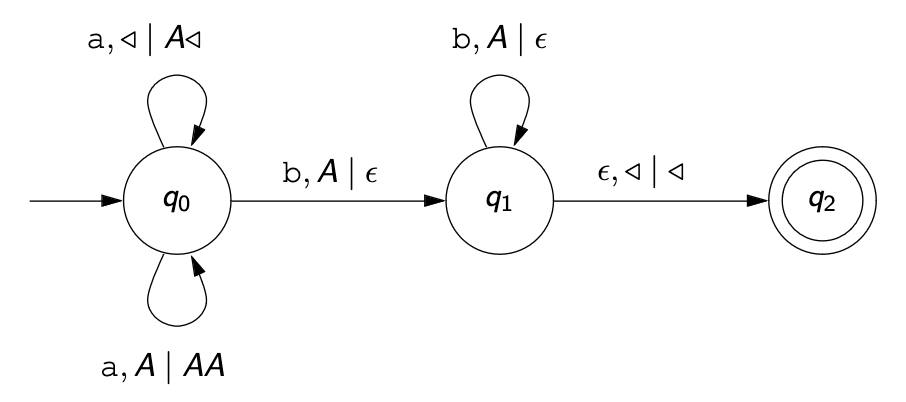
\includegraphics[width=\columnwidth]{context-free-2}
\end{figure}
The empty string $\epsilon$ can be used as an input symbol. This is useful to detect that the stack 
is empty.\\

\textit{Example: } A PDA that recognizes $L = \{a^n b^{2n} | n \geq 1\}$ could be:
\begin{figure}[H]
  \centering
  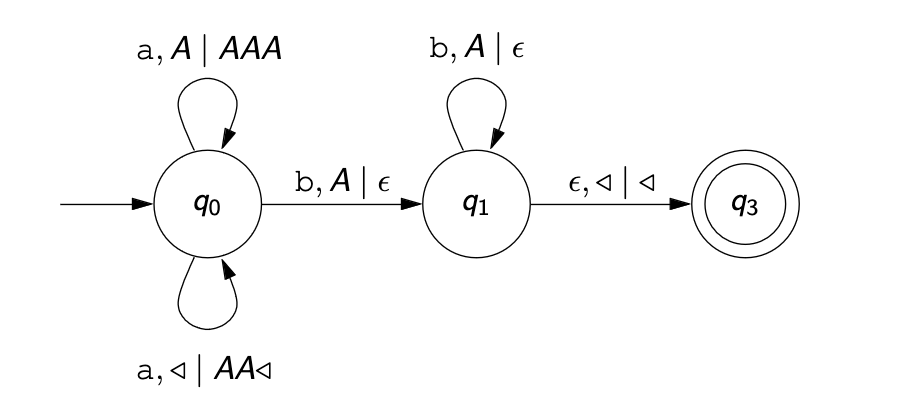
\includegraphics[width=\columnwidth]{context-free-3}
\end{figure}
\subsubsection{Limitations of PDA}
The language $L = \{a^n b^m | m = n \text{ or } mm = 2n\}$ cannot be recognized
by a PDA with a single stack. It would require two stacks, where the first 
stack would recognize the number $n$ and the second one would recognize the number $2n$.

\subsubsection{Non-deterministic PDA}
Non-determinism is modeled by means of a transition function whose co-domain is a power set.
The formal definitions is as follows: A non-deterministic PDA is a 7-tuple $M = (Q,\Sigma,\Gamma,\delta,q_0,\triangleleft)$
with $\delta: Q \times (\Sigma \cup \{\epsilon\}) \times \Gamma \rightarrow \mathcal{P}(Q \times \Gamma^{*})$
where $\mathcal{P}(Q \times \Gamma^{*})$ denotes the power set of $Q \times \Gamma^{*}$.
A word is recognized by a non-deterministic PDA iff there is at least one path between the 
initial state and a final state.\\

It is important to observe that the classes of languages recognized by deterministic and non-deterministic
PDA are not the same.
Non-deterministic PDA recognize a larger class of languages than deterministic PDA, i.e. they are more powerful.
This is not the case for FSAs.
\subsection{Context-free Grammars}
The difference between regular grammars 
and \textbf{context-free} grammars is the restrictions imposed on the rewriting rules.
The rules of regular grammars are more restrictive than the ones of context-free grammars, 
which means that any regular grammar is also a context-free grammar. Context-free grammars
have a greater expression power than regular ones.\\

The formal definition of context-free grammars is as follows:
A context-free grammar $G = (V_T, V_N, P, S)$ is a grammar 
whose productions have the form $\alpha \rightarrow \beta$, where 
\begin{enumerate}
  \item $\lvert \alpha \rvert = 1$ and $\alpha \in V_N$
  \item $\beta$ is a sequence of terminal and/or non-terminals
\end{enumerate}
The language generated by a context-free grammar $G$ is called a \textbf{context-free} language,
denoted by $L(G)$.\\

\textit{Example:} Let $L = \{a^n b^n \mid n \geq 1\}$. The grammar that generates $L$ can be defined as:
\begin{align*}
  G = (\{a,b\}, \{S\}, P, S)
\end{align*}
where $P= \{S \rightarrow aSb, S \rightarrow ab\}$\\

\textit{Example:} Let G = (\{a,b\}, \{S,A,B\}, P, S)
with 
\begin{align*}
  P = \{ & S \rightarrow aB,\\
    & S \rightarrow bA,\\
    & A \rightarrow a,\\
    & A \rightarrow aS,\\
    & A \rightarrow bAA,\\
    & B \rightarrow b,\\
    & B \rightarrow bS,\\
    & B \rightarrow aBB
    \}
\end{align*}
$G$ is context-free and generates the language of all words composed of the same number of symbols $a$ and $b$.

\subsection{BNF}
The \textbf{Backus-Naur Form} (BNF) is a notation used to describe 
the syntax of programming languages (originally Algol 60). BNF uses ASCII
characters only and is equivalent to the notion of context-free grammars.
\begin{itemize}
  \item Non-terminals are strings, e.g. \texttt{type}, \texttt{identifier}, etc.
  \item Terminals are (single or double) quoted strings or symbols, such as \texttt{"while", "float", 's', '+'}, etc.
  \item = corresponds to the arrow of a production $\alpha \rightarrow \beta$
  \item $\mid$ corresponds to alternative
  \item , concatenates elements
  \item ; terminates a production
\end{itemize}
The extended BNF (EBNF) is similar, but introduces some new constructs 
that make the notation easier to read and more compact. The most immporant aspects of EBNF are:
\begin{itemize}
  \item Parantheses can be used to group elements
  \item \texttt{[} $\gamma$ \texttt{]} means that $\gamma$ is optional, i.e. appears zero or one times.
  \item \texttt{\textbraceleft} $\gamma$ \texttt{\textbraceright} means that $\gamma$ can be repeated zero or more times.
\end{itemize}

\subsection{Parse Trees, Ambiguity}
The application of rewriting rules captures the notion of the \textbf{parse tree}.
For some grammars, a word can be generated in several different ways and have thus 
several different parse trees. Such words are generated ambiguously and may potentially 
have several different meanings.
Having different meanings is sometimes undesirable, especially in the context of programming languages,
where a given program should have unique semantics.\\

\textit{Example: } Consider the productions $S \rightarrow AAB, A \rightarrow aAa, A \rightarrow a,
B \rightarrow b$. There are several ways of generated the string $aaaab$, e.g.
\begin{figure}[H]
  \centering
  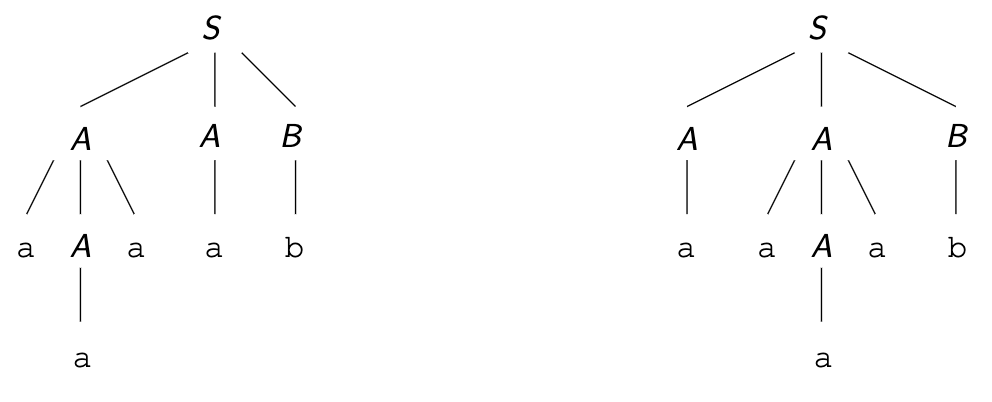
\includegraphics[width=\columnwidth]{context-free-4}
\end{figure}
The definition of an ambiguous grammar is as follows:
A grammar $G$ is an ambiguous grammar iff there exists a word  
$w \in L(G)$ such that $w$ has more than one parse tree.
A language $L$ is an ambiguous language iff all the grammars that generate $L$ are ambiguous.\\

The theorem for PDA and context-free languages is as follows:
A language $L$ is recognized by a non-deterministic PDA iff $L$ is a context-free language.